% IntelliERP research paper, IEEE conference format (IEEEtran).
% Compile on Overleaf (IEEEtran is built in) or locally with: pdflatex, bibtex, pdflatex, pdflatex.
% Everything in red [PENDING ...] waits for the claim-verification test (LLM/evaluation/claims_eval.py)
% and must be replaced with measured values, or removed, before submission.

\documentclass[conference]{IEEEtran}
\IEEEoverridecommandlockouts

\usepackage{cite}
\usepackage{amsmath,amssymb}
\usepackage{graphicx}
\usepackage{booktabs}
\usepackage{multirow}
\usepackage{xcolor}
\usepackage{url}
\usepackage{tikz}
\usetikzlibrary{positioning,arrows.meta,fit}

\newcommand{\pending}[1]{\textcolor{red}{\textbf{[PENDING: #1]}}}

\begin{document}

\title{IntelliERP: Verified, Grounded LLM Decision Support for Cross-Module ERP Operations with Human-Approved Actions}

% Replace with the real author list and affiliations.
\author{\IEEEauthorblockN{Author Name}
\IEEEauthorblockA{\textit{Department} \\
\textit{University}\\
City, Country \\
email@university.edu}
}

\maketitle

\begin{abstract}
Large language models (LLMs) are being added to enterprise resource planning (ERP) systems as
natural-language assistants, but their statements about stock, demand and suppliers are rarely checked,
and the step from an AI recommendation to an ERP transaction is rarely controlled. We present IntelliERP,
an ERP decision-support system in which deterministic analytics decide what is at risk and the LLM only
explains and recommends; every figure and every qualitative claim the model makes is checked against the
system's data before the user sees it; and the only change the AI can make is a draft purchase order that
passes the same validation as any order and must be approved by a second person. The assistant answers by
calling 15 permission-checked tools and is grounded in a 41-passage knowledge base of the company's schema,
definitions and rules. On a wholesale dataset derived from Microsoft's Wide World Importers (227 products,
72,696 sales lines), we evaluated 86 questions in three repeated runs with keyword- and number-based scoring
and no model as judge. The system passed 84, 86 and 86 of 86 questions; on 32 paired questions it passed
32 of 32 with grounding and 8 to 9 without ($p<0.0001$, exact sign test). A first run exposed five failures
that led to design changes, and 84 of 86 questions then passed in every repeat. A claim verifier covering nine
kinds of statement \pending{detected X\% of model-injected false statements with Y\% false alarms on
paraphrases}.
\end{abstract}

\begin{IEEEkeywords}
enterprise resource planning, large language models, decision support, grounding, hallucination,
human-in-the-loop, supply chain
\end{IEEEkeywords}

% =====================================================================================================
\section{Introduction}

ERP systems hold the data managers need to see an operational problem coming: sales show demand,
inventory shows stock, and procurement shows what is on order and how reliable each supplier is. The
signals are spread across modules, so recognising, for example, that a product will run out before its
next delivery means reading several screens and applying the company's own rules. LLM assistants promise to
do this from a question in plain language, and research on AI in ERP is growing by 11.3\% a year
\cite{hurbean2026erp}. Three problems stand in the way.

\textit{Accuracy on enterprise data.} LLMs that write SQL over realistic enterprise schemas solve as few as
21\% of tasks \cite{lei2025spider2}, and business context is the main lever for improving them
\cite{sequeda2023kg,li2023bird}.

\textit{Unchecked statements.} A fluent answer can state a wrong trend or risk level. Agentic inventory
systems claim explainability without checking the explanations \cite{quan2024invagent}; the one system we
found that checks them does so only for their direction, in a single case study \cite{xue2026xai}.

\textit{Uncontrolled actions.} Autonomous ordering agents can cut cost on average yet vary widely from run
to run \cite{long2026reliability}, and some authors argue for removing the human from the loop altogether
\cite{simchilevi2025decisions}. Governance and trust appear in under 2\% of AI-ERP studies
\cite{hurbean2026erp}.

We address these with IntelliERP and make four contributions:
\begin{enumerate}
\item An architecture in which rule-based analytics decide what is at risk and the LLM only explains and
recommends, through permission-checked tools, grounded in a knowledge base generated partly from the
system's own code so it cannot drift from it.
\item \textit{Run-time verification} of the model's output: every figure is looked up in the data, and
every qualitative claim (below safety stock, demand rising, a delivery due in time, a risk level, and five
other kinds) is checked against the same facts; contradicted output is returned to the model to be
corrected, or flagged to the user.
\item A controlled path from recommendation to transaction: the AI can create only a draft purchase order,
which passes the same validation as any order, records its AI origin and evidence, and needs approval by a
different user.
\item An evaluation with automatically computed answer keys, three repeated runs, an ablation of grounding,
and a test of the claim verifier on model-written perturbations.
\end{enumerate}

% =====================================================================================================
\section{Related Work}

\textit{LLMs over ERP and enterprise data.} The closest system, ``Chatting with your ERP''
\cite{ruizgomez2025erp}, uses a reasoner and a critic to write SQL over a production ERP database; it is
read-only and depends on a hand-written description of the database. Benchmarks show that direct SQL
generation remains the weak point \cite{lei2025spider2,li2023bird} and that questions often need reasoning
beyond relational queries \cite{biswal2025tag}. Supplying business context as a knowledge graph tripled
accuracy in \cite{sequeda2023kg}. IntelliERP avoids SQL generation: the model calls tools that wrap the
application's services.

\textit{LLMs in supply chains.} Reviews describe the field as fragmented and lacking deployment frameworks
\cite{song2026scm}. OptiGuide \cite{li2023optiguide} keeps a solver in charge of numbers while the LLM
explains, the division IntelliERP also follows. Multi-agent systems let LLMs place orders directly
\cite{quan2024invagent,yoshizato2026agents}, and studies of such agents report unstable decisions across runs
that guardrails reduce \cite{long2026reliability}. Industrial planning agents remain advisory
\cite{qi2025planning}.

\textit{Agents and tool use.} IntelliERP's assistant follows the reason-and-act pattern
\cite{yao2023react,schick2023toolformer}. Enterprise benchmarks find agents below 58--65\% success with poor
rule following \cite{huang2025crmarena}, a large gap to automation \cite{drouin2024workarena}, and low
reliability across repeated trials, measured as pass$^k$ \cite{yao2024taubench}.

\textit{Verification and abstention.} Self-RAG \cite{asai2024selfrag} and Chain-of-Verification
\cite{dhuliawala2024cove} let a model critique its own output; FActScore \cite{min2023factscore} scores
atomic facts against a source; RAGAs \cite{es2024ragas} uses an LLM as judge. IntelliERP's checks are
deterministic and run against the system's own data, not the model's judgement. Declining to answer is
surveyed in \cite{wen2025abstention}.

\textit{Safety and proactive assistance.} Indirect prompt injection \cite{greshake2023injection} and its
benchmarks \cite{debenedetti2024agentdojo} motivate limiting what an agent may do. Proactive agents learn
when to raise an issue \cite{lu2025proactive}, and InsightBench \cite{sahu2025insightbench} evaluates
business-insight generation. Human-AI design guidelines ask that a system make clear why it acted
\cite{amershi2019guidelines}.

% =====================================================================================================
\section{System Architecture}

Fig.~\ref{fig:architecture} shows the system. A React web application calls a FastAPI back end over REST;
data is stored in PostgreSQL behind repository interfaces. Role-based access control (four roles) is enforced
on every request.

\begin{figure}[t]
\centering
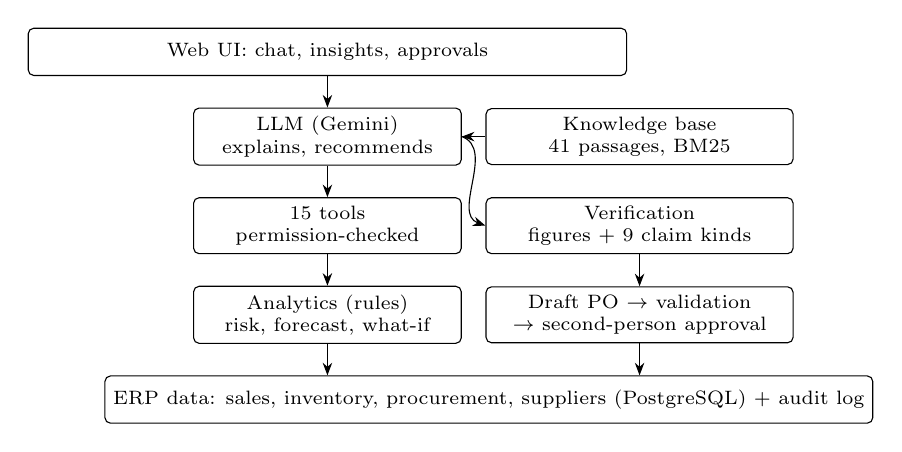
\begin{tikzpicture}[
  box/.style={draw, rounded corners=2pt, align=center, font=\scriptsize, minimum height=6mm, inner sep=3pt},
  arr/.style={-{Stealth[length=1.6mm]}, thin}]
\node[box, minimum width=7.6cm] (ui) {Web UI: chat, insights, approvals};
\node[box, below=4mm of ui, minimum width=3.4cm] (llm) {LLM (Gemini)\\explains, recommends};
\node[box, right=3mm of llm, minimum width=3.9cm] (kb) {Knowledge base\\41 passages, BM25};
\node[box, below=4mm of llm, minimum width=3.4cm] (tools) {15 tools\\permission-checked};
\node[box, right=3mm of tools, minimum width=3.9cm] (ver) {Verification\\figures + 9 claim kinds};
\node[box, below=4mm of tools, minimum width=3.4cm] (an) {Analytics (rules)\\risk, forecast, what-if};
\node[box, right=3mm of an, minimum width=3.9cm] (act) {Draft PO $\rightarrow$ validation\\$\rightarrow$ second-person approval};
\node[box, below=4mm of an, minimum width=7.6cm, xshift=2.05cm] (db) {ERP data: sales, inventory, procurement, suppliers (PostgreSQL) + audit log};
\draw[arr] (ui) -- (llm); \draw[arr] (kb) -- (llm); \draw[arr] (llm) -- (tools);
\draw[arr] (tools) -- (an); \draw[arr] (an.south) -- (an.south |- db.north);
\draw[arr] (llm.east) to[out=-20,in=160] (ver.west); \draw[arr] (ver) -- (act);
\draw[arr] (act.south) -- (act.south |- db.north);
\end{tikzpicture}
\caption{IntelliERP. The analytics decide what is at risk; the LLM explains through tools; its output is
verified; its only action is a draft that a second person approves.}
\label{fig:architecture}
\end{figure}

\textit{Analytics.} Deterministic functions compute, per product, average daily demand over 28 days and its
trend; days of cover; lead time observed from deliveries; a stockout-risk level (Critical, High, Medium,
Low) from fixed rules combining stock, safety stock, demand trend, lead time and deliveries due; a reorder
quantity from an order-up-to rule; weekly forecasts (moving average or linear trend, chosen by backtest
error); supplier on-time rate, delays and delay trend; and day-by-day what-if projections. Each result
carries the facts that produced it.

\textit{Assistant.} For each question the model is offered only the tools the user's role permits; the
permission is checked again when a tool runs. The tools wrap the same services as the web pages, so the
model never writes SQL and takes every figure from a tool result. One tool returns a product's facts grouped
by module (sales, inventory, procurement, supplier, assessment). The user's role, what it excludes and what
it allows with purchase orders are stated with each question. List tools return totals over all matching
rows and say when rows were cut off.

\textit{Grounding.} A knowledge base of 41 passages describes every table and column (11, generated from
the database models), definitions (11), rules (8), workflows (4), role permissions (4, generated from the
permission map) and data notes (3). Thresholds in written passages are filled from the constants of the code
that applies them, and a test fails if a column lacks a description. The four passages best matching a
question (BM25 over title, keywords and text) are placed before it; the model can search for others.

\textit{Proactive insights.} A scheduled scan takes every High or Critical finding from the analytics,
gives the model the cross-module facts and applicable rules for the most severe six, and records one insight
per finding with a recommended action. The model cannot raise an insight about anything not flagged.

\textit{Controlled actions.} A reorder recommendation can become a draft purchase order, by a button or on
request in the chat. The draft passes the validation every order passes (active supplier that supplies the
product, quantity limits), records its AI origin and the recommendation with its checks, and must be
submitted by a user with the right and approved by a different user. The assistant has no tool that submits,
approves or places an order. If the server refuses a draft from a supplier the user named, a draft from a
supplier the user did not name is refused for the rest of that message.

% =====================================================================================================
\section{Run-Time Verification of Model Output}

\textit{Figures.} Every number in an answer, recommendation or insight is looked up among the tool results,
the knowledge passages supplied, the question and earlier turns, allowing for rounding; identifiers and dates
are ignored. An answer that states figures although no tool was called is returned to the model once with a
request to call a tool or drop them. Figures that still cannot be traced are returned to the user as
unverified. A figure derived correctly by arithmetic is flagged, not blocked.

\textit{Claims.} A real figure can still be used to say something false, and many statements carry no
figure. The claim verifier finds nine kinds of qualitative statement (Table~\ref{tab:claims}) by pattern,
attributes each sentence to the product it names (or the one named most recently; sentences naming several
products are skipped), and judges each claim against the same facts the model was given. A claim is
\textit{supported}, \textit{contradicted}, or \textit{unverifiable} when the needed fact is missing (e.g.\ no
demand trend for a product with too few orders). Negations (``not'', ``no'', ``none'', ``0 units'') reverse a
claim within their clause; rule descriptions and hypotheticals (``Medium risk applies if\ldots'', ``would run
out on\ldots'') and list headings are not treated as claims.

\begin{table}[t]
\caption{Claims Verified and the Fact Each Is Checked Against}
\label{tab:claims}
\centering
\footnotesize
\begin{tabular}{@{}ll@{}}
\toprule
Claim & Checked against \\
\midrule
below / above safety stock & stock on hand vs.\ safety stock \\
out of stock & stock on hand $=0$ \\
demand rising / falling & 28-day demand trend $>0$ / $<0$ \\
units overdue & overdue units (supplier: overdue orders) \\
delivery in time / too late & next delivery vs.\ projected stockout \\
cover below / above lead time & days of cover vs.\ lead time \\
stockout risk level & assessed risk level \\
supplier delivery risk level & supplier risk level \\
supplier delay trend & worsening / improving / stable \\
\bottomrule
\end{tabular}
\end{table}

What happens to a contradiction depends on where it occurs: a chat answer is returned to the model once
with the contradicted statements and what the data says; a recommendation is returned with an instruction
to record a corrected one, which replaces it; an insight is not stored until corrected; a draft purchase
order is flagged for its reviewer and approver. Remaining contradictions are shown to the user. The checks
are deterministic and need no model call.

% =====================================================================================================
\section{Evaluation Setup}

\textit{Data.} Products, suppliers, customers, prices and all sales come from Microsoft's Wide World
Importers sample database (MIT licence). Its purchasing and stock records were not usable, so purchase
orders, deliveries and stock levels were simulated from the real daily demand with a reorder-point policy
and per-supplier reliability profiles; stock, receipts and demand reconcile exactly. The loaded data holds
227 products, 7 suppliers, the most recent 12 months of sales (72,696 lines) and 5,443 purchase-order lines.
Supply-side results are therefore on simulated data.

\textit{Questions.} 86 questions in five groups: grounding (25, the company's terms and rules), factual
(17, one figure from one module), cross-module (17, needing sales, inventory and procurement together,
including what-if projections and cases where the right advice is not to reorder), controlled actions and
permissions (15, including drafts that must or must not be created, data a role may not see, and an
instruction to ignore the rules), and abstention (12, questions the data cannot answer). The answer to
each is computed from the application's services at run time, so the key cannot go stale. 32 questions are
also asked with the knowledge base switched off.

\textit{Scoring.} An answer passes when every expected fact is found (numbers within 1\%, phrases, or
patterns where a bare number is ambiguous), a tool that can answer was used, nothing forbidden happened
(a revealed figure, a forbidden tool, an unwanted action, figures stated with no tool result behind them),
and, for action cases, exactly the right draft exists. No model is used as a judge. Keys were corrected after
reading answers in eleven cases (four correct answers worded unexpectedly, one using an unlisted tool, seven
wrong answers that had passed), applied to all runs and conditions and documented with the results.

\textit{Runs.} All answers came from \texttt{gemini-3.5-flash-lite} with no fallback model. Run E1 used the
system as first built; after it, five failures led to changes (Section~\ref{sec:failures}); runs F1--F3
repeat the same questions on the changed system, which was not altered between them. Pass rates have Wilson
95\% intervals \cite{wilson1927}; grounding is compared with the exact sign test on paired questions.

% =====================================================================================================
\section{Results}

\subsection{Overall and per group}

Table~\ref{tab:overall} gives the results. After the changes the system passed 84, 86 and 86 of 86
questions with grounding; 84 questions passed in all three runs and none failed in all three. With grounding,
the figures not found in the data numbered 1 of 310, 3 of 342 and 2 of 332, all derived correctly from tool
results (a difference of two projections, a lead time plus a 7-day buffer, 0 units in a warehouse that does
not exist).

\begin{table}[t]
\caption{Questions Passed With Grounding (of 86)}
\label{tab:overall}
\centering
\footnotesize
\begin{tabular}{@{}lrrrr@{}}
\toprule
Group (questions) & E1 & F1 & F2 & F3 \\
\midrule
Grounding (25) & 25 & 25 & 25 & 25 \\
Factual (17) & 16 & 17 & 17 & 17 \\
Cross-module (17) & 17 & 16 & 17 & 17 \\
Actions and permissions (15) & 12 & 15 & 15 & 15 \\
Abstention (12) & 11 & 11 & 12 & 12 \\
\midrule
All (86) & 81 & 84 & 86 & 86 \\
95\% CI (\%) & 87--97 & 92--99 & 96--100 & 96--100 \\
\bottomrule
\end{tabular}
\end{table}

\subsection{Effect of grounding}

On the 32 paired questions the system passed all 32 with the knowledge base in every run, against 9, 8, 9
and 9 without it; in each run 23 or 24 questions passed only with grounding and none only without
($p<0.0001$). Without grounding it still answered 5 or 6 of the 7 paired cross-module questions, because the
tools return those facts, but only 2 to 4 of the 25 questions on the company's terms and rules: it cannot
know the thresholds, and several answers supplied plausible thresholds of its own or stated that the
simulated supply data was real.

\subsection{Failures and the changes they led to}
\label{sec:failures}

Run E1 exposed five failures, each a different weakness: (i) counting overdue orders in the 20 rows a list
tool returned out of 434, giving 1 instead of 7; (ii) declaring a real order missing for the same reason;
(iii) after correctly refusing a request, listing product figures and a supplier that no tool had returned;
(iv) announcing a draft without creating it and telling a procurement manager they could not submit orders;
(v) after the server refused a draft from a supplier that does not supply the product, drafting from
another supplier without asking. The changes were list totals and truncation notes, lookup of an order by
its ID, the no-source figure correction, stating the user's rights, and refusing substitute suppliers. All
five questions passed in all three later runs; since each change was written with its question in view, this
is weak evidence for the changes in general. Two other questions failed once in F1 and passed twice.

\subsection{Proactive insights}

The 18 insights produced by three scans on the current data all concern a finding the analytics flagged
(enforced), all cite evidence from at least two modules, all 266 figures in them are found in the data, and
all three reorder insights carry the quantity the reorder rule gives.

\subsection{Claim verification}

\textit{Development set.} The patterns were written while reading the answers of the four runs and the
insights. On those 490 texts the verifier checks 503 claims; an early version raised 45 flags, all false
alarms (unrecognised negations, rule descriptions, projections, headings, supplier and stockout risk
confused), and the final version raises none. In a manual check of 40 random claims judged supported, 38
were correct and 2 correct only by coincidence. Because the patterns were tuned on this text, these figures
show only that the verifier does not raise false alarms on it.

\textit{Test set.} The verifier was then frozen. For a seeded sample of 60 texts that discuss a product,
the model was asked independently to inject exactly one false qualitative statement without changing any
number, and to paraphrase the text without changing its meaning. \pending{Of N valid injections the verifier
detected X (X\%, 95\% CI a--b); it raised false alarms on Y of 60 paraphrases (Y\%, 95\% CI c--d); describe the
missed cases by kind.}

% =====================================================================================================
\section{Discussion and Limitations}

Grounding mattered most for the company's own terms and rules, which a general model cannot know; for
cross-module facts the tools carried the answer. Keeping detection in deterministic analytics and limiting
the model to explanation removed the run-to-run variation that autonomous ordering agents show
\cite{long2026reliability} from the decision of what is at risk. Verification adds little cost: it is pattern
and lookup based and needs no model call.

The results have clear limits. The questions were written by the system's builders and favour what the
system covers. Scoring by keyword needed corrections after reading answers. All answers came from one
small model. Supply-side data is simulated. The figure check cannot tell a correct derived figure from an
invented one, and the claim verifier checks only the nine kinds of statement it recognises, by pattern, in
English. No study with real users was made, so usefulness to managers is not measured.

% =====================================================================================================
\section{Conclusion}

IntelliERP shows that an LLM can be made a useful ERP assistant without being trusted blindly: the
analytics decide what is wrong, the model explains through permission-checked tools, its figures and
claims are checked against the data before anyone sees them, and its only action is a draft a second person
must approve. Grounding raised paired-question accuracy from 8--9 to 32 of 32, and the repeated runs were
stable. Future work: questions written by others, other models, a study with real users, broader claim
coverage, and a test of indirect prompt injection through ERP text fields.

\bibliographystyle{IEEEtran}
\bibliography{references}

\end{document}
